\documentclass{beamer}
\usepackage{graphicx}
\usepackage{epstopdf}
\usepackage{hyperref}
\usepackage{tikz}
\usepackage{listings}
\usepackage{subfig}

\usetikzlibrary{
    chains,
    positioning,
    arrows.meta,
    decorations.pathreplacing,
    calc,
    fit,
    shapes.geometric
}
                    
\graphicspath{ {images/} }

\bibliographystyle{plain}

\usetheme{Boadilla}

% https://latex.org/forum/viewtopic.php?t=6662
\setbeamertemplate{footline}
{
   \leavevmode%
   \hbox{%
   \begin{beamercolorbox}[wd=.333333\paperwidth,ht=2.25ex,dp=1ex,center]{author in head/foot}%
     \usebeamerfont{author in head/foot}\insertshortauthor%~~(\insertshortinstitute)
   \end{beamercolorbox}%
   \begin{beamercolorbox}[wd=.333333\paperwidth,ht=2.25ex,dp=1ex,center]{title in head/foot}%
     \usebeamerfont{title in head/foot}\insertshorttitle
   \end{beamercolorbox}%
   \begin{beamercolorbox}[wd=.333333\paperwidth,ht=2.25ex,dp=1ex,right]{date in head/foot}%
     \usebeamerfont{date in head/foot}\insertshortdate{}\hspace*{2em}
     \insertframenumber{} / \inserttotalframenumber\hspace*{2ex}
   \end{beamercolorbox}}%
   \vskip0pt%
}

\title{CS4099 Demo}
\subtitle{Ubiquitous Communication for the Internet of Things\\An Identifier-Locator addressing split overlay network}
\author{Ryan Gibb}
\institute{School of Computer Science\\University of St Andrews}
\titlegraphic{\includegraphics[scale=2,trim={0.45cm 0.75cm 0.45cm 0.45cm},clip]{st_a_logo.eps}}

\date{Monday 19th April}

\AtBeginSection[]{
  \begin{frame}
  \vfill
  \centering
  \begin{beamercolorbox}[sep=8pt,center,shadow=true,rounded=true]{title}
    \usebeamerfont{title}\insertsectionhead\par%
  \end{beamercolorbox}
  \vfill
  \end{frame}
}

\begin{document}

\begin{frame}
	\maketitle
\end{frame}

\begin{frame}{Background}
\begin{itemize}
    \item Ubiquitous Computing and the Internet of Things (IoT)
    \pause
    \item Mobility in IP
    \pause
    \begin{itemize}
        \item Overloading of IP address semantics
        \item Entanglement of layers
    \end{itemize}
    \pause
    \item Identifier-Locator Network Protocol (ILNP)
\end{itemize}
\end{frame}

\begin{frame}{An Identifier-Locator Overlay Network}
\begin{itemize}
    \item Userspace and Python
    \pause
    \item Focus on protocol design and interaction
    \pause
    \item Evaluated with experimental analysis in IoT (Raspberry Pis)
\end{itemize}
\end{frame}

\begin{frame}{Overlay Network Stack}
\begin{figure}[ht]
    \centering
    \scalebox{0.75}{
% Adapted from
% https://tex.stackexchange.com/questions/468410/tikz-drawing-layer-by-layer

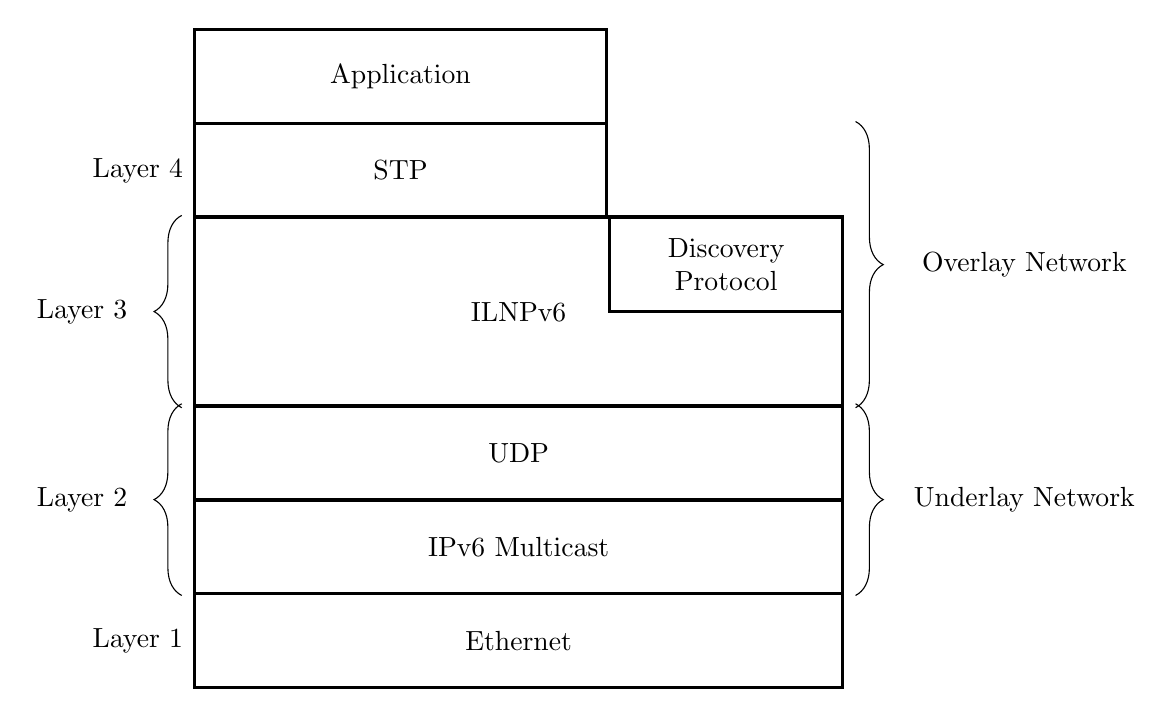
\begin{tikzpicture}[
    node distance = -0.5mm and 0mm,
    start chain = going below,
    layer/.style args = {#1}{
        rectangle, draw, very thick,
        text width=8cm, align=center,
        minimum height=12mm,
        label=left:#1
    }
]

    % \node (n3) [layer={Layer 3}, on chain] {ILNPv6};
    %     \node (n4) [layer={Layer 4},above right=of n3.north west,text width=5cm] {STP};
    %     \node (n5) [layer={Layer 7},above right=of n4.north west,text width=5cm] {Application: Experiments/Heartbeat};
    %     \node (n4B) [layer=,above left=of n3.north east,text width=2cm] {Discovery Protocol};
    %     \node (n5B) [layer=,above left=of n4B.north east,text width=2cm,draw=none] {};
    % \node (n3) [layer={}, on chain] {ILNPv6};
    %     \node (n3A) [layer={},above right=of n3.north west,text width=5cm] {};
    %     \node (n4) [layer={Layer 4},above right=of n3A.north west,text width=5cm] {STP};
    %     \node (n5) [layer={Layer 7},above right=of n4.north west,text width=5cm] {Application: Experiments/Heartbeat};
    %     \node (n3B) [layer=,above left=of n3.north east,text width=2cm] {Discovery Protocol};
    %     \node (n4B) [layer=,above left=of n3B.north east,text width=2cm,draw=none] {};
    %     \node (n5B) [layer=,above left=of n4B.north east,text width=2cm,draw=none] {};
    \node (n3) [layer={}, on chain, minimum height=24mm] {ILNPv6};
        \node (n4) [layer={Layer 4},above right=of n3.north west,text width=5cm] {STP};
        \node (n5) [layer={},above right=of n4.north west,text width=5cm] {Application};
        \node (n3B) [layer=,below left=0pt and 0pt of n3.north east,text width=2.73cm] {Discovery Protocol};
        \node (n4B) [layer=,above left=of n3B.north east,text width=2cm,draw=none] {};
        \node (n5B) [layer=,above left=of n4B.north east,text width=2cm,draw=none] {};
    
    \node (n2) [layer, on chain] {UDP};
    \node (n1) [layer, on chain] {IPv6 Multicast};
    \node (n0) [layer={Layer 1}, on chain] {Ethernet};
    
    \draw [decorate, decoration={brace, amplitude=10pt, raise=4pt, mirror}]
        (n3.south east) -- (n4B.north east)
        node [black, midway, xshift=65pt] {Overlay Network};
    
    \draw [decorate, decoration={brace, amplitude=10pt, raise=4pt, mirror}]
        (n1.south east) -- (n2.north east)
        node [black, midway, xshift=65pt] {Underlay Network};
    
    \draw [decorate, decoration={brace, amplitude=10pt, raise=4pt}]
        (n1.south west) -- (n2.north west)
        node [black, midway, xshift=-40pt] {Layer 2};
    
    \draw [decorate, decoration={brace, amplitude=10pt, raise=4pt}]
        (n3.south west) -- (n3.north west)
        node [black, midway, xshift=-40pt] {Layer 3};

\end{tikzpicture}
}
    \caption{Overlay Network Stack}
    \label{fig:network_stack}
\end{figure}
\end{frame}



\begin{frame}{Discovery Protocol Example}
\begin{figure}[ht]
    \centering
    \makebox[\textwidth]{
        \begin{tabular}{c}            
            \subfloat[Network Topology \label{fig:discovery_topology}]
                {\scalebox{0.4}{\input{diagrams/discovery_protocol_topology.tex}}} \\
            \subfloat[Sequence Diagram \label{fig:discovery_sequence}]
                {\scalebox{0.4}{\input{diagrams/discovery_protocol_sequence_diagram.tex}}} \\
        \end{tabular}
    }
    \caption{Discovery Protocol Example}
    \label{fig:discovery}
\end{figure}
\end{frame}


\begin{frame}{Locator Update Example}
\begin{figure}[ht]
    \centering
    \makebox[\textwidth]{
        \begin{tabular}{cc}
            \subfloat[Network Topology \label{fig:locator_udpate_topology}]
                {\scalebox{0.35}{\input{diagrams/locator_update_topology.tex}}} &
            \subfloat[Sequence Diagram \label{fig:locator_update_sequence_diagram}]
                {\scalebox{0.35}{\input{diagrams/locator_update_sequence_diagram.tex}}} \\
        \end{tabular}
    }
    \caption{Locator Update Example}
    \label{fig:locator_udpate}
\end{figure}
\end{frame}

\begin{frame}{Physical Testbed}
\begin{figure}[ht]
    \centering
    \includegraphics[width = 0.75\textwidth]{testbed.jpg}
    \caption{Physical Testbed}
    \label{fig:physical_testbed}
\end{figure}
\end{frame}

\begin{frame}{Experiment Virtual Topology}
\begin{figure}[ht]
    \centering
    \scalebox{0.35}{\input{diagrams/experiment.tex}}
    \caption{Experiment Virtual Topology}
    \label{fig:experiment_topology}
\end{figure}
\end{frame}

\section{Heartbeat Demo}

\begin{frame}{Experiment Results}
\begin{figure}[p]
    \centering
    \makebox[\textwidth]{
        \begin{tabular}{cc}
            \subfloat[Received sequence numbers vs Time on MN \label{fig:exp3seqnos_mn}]{
                \includegraphics[width = 0.45\textwidth]{graphs/exp3/Received sequence numbers vs Time on MN.pdf}
            } &
            \subfloat[Received sequence numbers vs Time on CN \label{fig:exp3seqnos_cn}]{
                \includegraphics[width = 0.45\textwidth]{graphs/exp3/Received sequence numbers vs Time on CN.pdf}
            } \\
        \end{tabular}
    }
    \caption{Experiment 3 MN\textless-\textgreater CN: Received sequence numbers vs Time}
    \label{fig:exp3seqnos}
\end{figure}
\end{frame}

\begin{frame}{Experiment Results}
\begin{figure}[p]
    \centering
    \makebox[\textwidth]{
        \begin{tabular}{cc}
            \subfloat[Throughput in 1s buckets vs Time on CN \label{fig:exp3throughputs_cn}]{
                \includegraphics[width = 0.45\textwidth]{graphs/exp3/Throughput in 1s buckets vs Time on CN.pdf}
            } &
            \subfloat[Throughput in 1s buckets vs Time on MN \label{fig:exp3throughputs_mn}]{
                \includegraphics[width = 0.45\textwidth]{graphs/exp3/Throughput in 1s buckets vs Time on MN.pdf}
            } \\
        \end{tabular}
    }
    \caption{Experiment 3 MN\textless-\textgreater CN: Throughput in 1s buckets vs Time}
    \label{fig:exp3throughputs}
\end{figure}
\end{frame}

\section{Questions?}

\begin{frame}{System Stability Issues}
\begin{figure}[p]
    \centering
    \makebox[\textwidth]{
        \begin{tabular}{cc}            
            \subfloat[Received sequence numbers vs Time on MN \label{fig:sys_issues_exp3seqnos_mn}]{\includegraphics[width = 0.45\textwidth]
                {systems_issues_graphs/exp3/Received sequence numbers vs Time on MN.pdf}} &
            \subfloat[Received sequence numbers vs Time on CN \label{fig:sys_issues_exp3seqnos_cn}]{\includegraphics[width = 0.45\textwidth]
                {systems_issues_graphs/exp3/Received sequence numbers vs Time on CN.pdf}} \\
        \end{tabular}
    }
    \caption{System Issues Experiment 3 CN\textless-\textgreater MN\\ Received sequence numbers vs Time}
    \label{fig:sys_issues_exp3seqnos}
\end{figure}
\end{frame}

\begin{frame}{System Stability Issues}
\begin{figure}[p]
    \centering
    \makebox[\textwidth]{
        \begin{tabular}{cc}            
            \subfloat[Throughput in 1s buckets vs Time on CN \label{fig:sys_issues_exp3throughputs_cn}]{\includegraphics[width = 0.45\textwidth]
                {systems_issues_graphs/exp3/Throughput in 1s buckets vs Time on CN.pdf}} &
            \subfloat[Throughput in 1s buckets vs Time on MN \label{fig:sys_issues_exp3throughputs_mn}]{\includegraphics[width = 0.45\textwidth]
                {systems_issues_graphs/exp3/Throughput in 1s buckets vs Time on MN.pdf}} \\
        \end{tabular}
    }
    \caption{System Issues Experiment 3 CN\textless-\textgreater MN\\ Throughputs in 1s buckets vs Time}
    \label{fig:sys_issues_exp1throughputs}
\end{figure}
\end{frame}

\end{document}
